\documentclass[12pt,a4paper,final,oneside,onecolumn,titlepage]{article}
\usepackage{times}
\usepackage{geometry}
\usepackage{fancyhdr}
\usepackage{setspace}
\usepackage{natbib}
\usepackage{amssymb}
\usepackage{graphicx}
\usepackage{sectsty}
\usepackage[table,xcdraw]{xcolor}
\usepackage{polski}
\usepackage[utf8]{inputenc}
\usepackage[T1]{fontenc}
\usepackage[pagewise]{lineno}
\newgeometry{tmargin=2.5cm, bmargin=2.5cm, lmargin=2.5cm, rmargin=2.5cm}
\setlength{\parindent}{3in}
\setlength{\parskip}{0pt}
\linenumbers
\doublespacing
\sectionfont{\centering}
\renewcommand{\bibsection}{\section*{\large{\textbf{\textsc{\centering{Literatura}}}}}}

\begin{document}
\pagestyle{fancy}
\fancyhead{}
\fancyfoot{}
\chead{Rola platformy Instagram w odbiorze własnego wyglądu}
\rhead{\thepage}
\bibliographystyle{apalike}
\begin{titlepage}
  \thispagestyle{empty}
  \rhead{\thepage}
  \begin{center}
  \vspace*{1cm}
  \Large
  \textbf{\textsc{Rola platformy Instagram w odbiorze własnego wyglądu:\\ Badanie zależności między modyfikowaniem swojego wizerunku, a oceną postrzegania swojego ciała wśród kobiet\\}}
  \vspace{1.5cm}
  \textit{Sara Pasturczak, Aleksandra Popowska, Wiktor Warchałowski\\}
  Wydział Nauk o Zdrowiu, Gdański Uniwersytet Medyczny\\
  \vspace{3cm}
  Praca zaliczeniowa z przedmiotu Metodologia Badań Psychologicznych napisana pod kierunkiem dr Małgorzaty Basińskiej\\
  \vspace{3cm}
  Gdańsk, 24 Maja 2022
  \end{center}
\end{titlepage}
\begin{center}
  \vspace*{0.5cm}
  \large{\textbf{\textsc{Abstrakt}}}
\end{center}
\paragraph{}
Celem niniejszego artykułu jest zbadanie problematyki związanej z zależnością mediów społecznościowych i samoakceptacji. Artykuł ten sprawdza czy fakt modyfikacji zdjęć własnego wizerunku na platformie Instagram ma związek z poziomem zadowolenia z własnego ciała u młodych kobiet. Badanie zostało przeprowadzone na 76 losowo dobranych użytkowniczkach platformy Instagram, najpopularniejszego serwisu społecznościowego wśród osób młodych. Postrzeganie własnego ciała zostało opisane jako wynik polskiej adaptacji 10 itemowego kwestionariusza Body Appreciation Scale 2, zaś fakt modyfikacji lub jego brak był podstawą do przydzielenia badanych do dwóch grup, które zostały ze sobą porównane. Średnie oraz mediany porównanych grup nie różniły się od siebie, zaś test t studenta nie wykazał statystycznie istotnej różnicy pomiędzy grupami. Współczynnik d Cohena pokazał brak efektu. Z tego powodu przyjęta została hipoteza alternatywna mówiąca o braku zależności.\\
\textit{Słowa kluczowe: media społecznościowe, postrzeganie siebie, ocena ciała}
\newpage
\begin{center}
\section*{\large{\textbf{\textsc{Wstęp}}}}
\end{center}
\paragraph{}
W dzisiejszych czasach coraz więcej osób ma dostęp do internetu, a co za tym idzie - również do portali społecznościowych, które cieszą się ogromnym zainteresowaniem. Najpopularniejszym portalem wśród amerykańskich nastolatków jest Instagram. Pozwala on na kontakty z rówieśnikami, wymianę informacji, a także wyrażanie siebie \citep{longobardi_follow_2020}. Jednakże tak powszechne użycie mediów społecznościowych prowokuje u młodych osób zachowania koncentrujące się na dążeniu do statusu w sieci (ang. \textit{digital status seeking}), czyli dążenia do popularności w Internecie mierzonej ilością polubień, komentarzy, udostępnień i obserwatorów \citep{nesi_search_2019}. Takie działania często prowadzą do zachowań ryzykownych, a samo wystawienie się na tego typu sieciową rywalizację, pozwala badaczom wysunąć wniosek, że Instagram jest najbardziej szodliwym serwisem społecznościowym. Jego nadmierne używanie może prowadzić nawet do problemów psychicznych czy zaburzeń postrzegania swojego ciała \citep{royal_society_for_public_health_status_2017}. Oprócz samego udziału młodych osób w kształtowaniu treści mediów społecznościowych, na tworzenie ich zawartości mają również wpływ czynniki socjokulturowe \citep{giorgianni_consumer_2020}. Kultura zachodnia od wieków ma tendencję do uprzedmiatawiania kobiet, a także cały czas zwraca uwagę na ważność wyglądu zewnętrznego \citep{lyu_travel_2016}. Ze względu na tak utarte kulturowe stereotypy, większość środków masowego przekazu powiela je i tworzy wizerunek ideału szczupłego ciała. Promowanie idelanych modelek i nagradzanie tego typu wizerunku w mediach jest czymś powszechnym. Stanowi to często główny powód niezadowolenia młodych kobiet ze swojego ciała, co z kolei może prowadzić do zaburzeń odżywiania \citep{grabe_role_2008}. Problemy te wynikają z dążenia do perfekcyjnego wyglądu, w celu sprostania oczekiwaniom społeczeństwa. Aby stworzyć złudzenie idealnego ciała w mediach społecznościowych, kobiety modyfikują swoje zdjęcia i często stanowi to dla nich mechanizm radzenia sobie z brakiem akceptacji siebie \citep{lyu_travel_2016}. Duży wpływ na poczucie zadowolenia z własnego wyglądu ma również porównywanie się z innymi osobami. Zetknięcie się przez młode dziewczęta ze zmodyfikowanymi zdjęciami rówieśników prowadzi do sytuacji, w których postrzegają one siebie bardziej negatywnie. Natomiast zdjęcia, które nie są przez rówieśników w żaden sposób zmienione, nie są źródłem takich skłonności \citep{kleemans_picture_2018}. Pomimo wielu przeprowadzonych badań potwierdzających szkodliwość platformy Instagram istnieją i takie, które zaprzeczają jego krzywdzącemu wpływowi. \citet{mclean_selfies_2015} w swoim badaniu pokazali, że publikowanie swoich zdjęć może wpływać na młode kobiety dwojako - mogą one zawyżać ocenę na temat swojego ciała, lub przyczyniać się do niezadowolenia z własnego wyglądu. Wyniki te mogą zaprzeczać jakiejkolwiek zależności między oceną własnego ciała a korzystaniem z mediów społecznościowych. Z tego powodu, celem niniejszego artykułu jest sprawdzenie czy fakt modyfikacji zdjęć własnego wizerunku na platformie Instagram ma związek z poziomem zadowolenia z własnego ciała u młodych kobiet. Przyjęta została hipoteza, iż fakt modyfikacji zdjęć będzie występował częściej u osób posiadających niskie zadowolenie z własnego wyglądu. Wynika to z faktu, że modyfikacja zdjęć może być mechanizmem radzenia sobie przez niektórych z negatywną samooceną \citep{kleemans_picture_2018,lyu_travel_2016}. Oprócz tego na tworzenie fałszywego wizerunku w mediach społecznościowych wpływa internalizacja ideału szczupłej sylwetki, która koreluje z negatywną oceną własnego ciała \citep{blowers_relationship_2003}.
\begin{center}
\section*{\large{\textbf{\textsc{Metoda}}}}
\end{center}
\subsection*{\normalsize{\textbf{Osoby badane}}}
\paragraph{}
Uczestnicy zostali wybrani metodą doboru przypadkowego. Osoby te otrzymały link do internetowego kwestionariusza i dobrowolnie go wypełniły. Łącznie kwestionariusz wypełniło 91 osób w wieku pomiędzy 18 a 25 rokiem życia. Jednakże 5 osób zaznaczyło płeć inną niż żeńska, 2 inne osoby zaś przyznały, że nie mają konta na platformie Instagram. Aby wypełnić założenia badania, osoby te (łącznie 7) zostały odrzucone z próby. W założeniach badania przewidziane było badanie osób łącznie z próbą kontrolną (osób, które nie publikują zdjęć swojego wizerunku) jednakże, ze względu na małą ilość takich osób (8) zostały one odrzucone - porównywalność i reprezentatywność grup nie zostałaby zachowana. Ostatecznie próba badana wyniosła 76 uczestników. Osoby badane w znacznej części pochodziły z miast o populacji powyżej 100 tys. mieszkańców. Były to również w większości jednostki pobierające naukę.
\subsection*{\normalsize{\textbf{Etyka}}}
\paragraph{}
Zgoda etyczna na przeprowadzenia badania została otrzymana od prowadzącego przedmiot Metodologia Badań Psychologicznych, realizowanym na Gdańskim Uniwersytecie Medycznym. Zarówno wykorzystany przez nas kwestionariusz, jak i sama metoda badania nie budzą żadnych etycznych wątpliwości. Kwestionariusz nie zbiera danych wrażliwych, a jego autorzy wyrazili pełną zgodę na użycie go przez nas w ramach zajęć prowadzonych na naszej uczelni. Uczestnicy zostali poinformowani o celu badania oraz o jego naturze. Zapewniono ich również, iż udział w badaniu jest zupełnie dobrowolny i w każdej chwili mogą z niego zrezygnować, przez cały czas pozostając anonimowym. Pozyskane zostało też potwierdzenie, że wszyscy uczestnicy ukończyli 18 lat i mają prawo do wyrażenia samodzielnej, świadomej zgody na udział w badaniu. 
\subsection*{\normalsize{\textbf{Zastosowane narzędzia i operacjonalizacja}}}
\paragraph{}
Zmienna niezależna, jaką jest modyfikowanie lub niemodyfikowanie zdjęć publikowanych na platformie Instagram została zoperacjonalizowana jako twierdząca lub przecząca odpowiedź na pytanie dotyczące modyfikacji zdjęć w brzmieniu ,,Czy kiedykolwiek, w jakikolwiek sposób zmodyfikowałaś zdjęcie swojego wizerunku na platformie Instagram tak, aby prezentować się na nim lepiej (prosimy o nieuwzględnianie filtrów, które jedynie zmieniają kolory na zdjęciach)?''. Zmienna zależna, jaką jest postrzeganie swojego ciała, została zoperacjonalizowana jako wynik kwestionariusza Body Appreciation Scale 2 (BAS-2) T. Tylka i N. Wood-Barcalow w polskiej adaptacji M. Razmus i W. Razmus. Wyższy wynik sumaryczny uzyskany przez odpowiedzi na pytania w pięciostopniowej skali Likerta jest interpretowany jako lepsze postrzeganie swojego ciała i posiadanie wyższej samooceny \citep{razmus_evaluating_2017,tylka_body_2015}.
\subsection*{\normalsize{\textbf{Procedura badania}}}
\paragraph{}
Badanie kwestionariuszowe zostało przeprowadzone przez Internet za pomocą Kwestionariuszy Google. Każdy badany musiał udzielić zgody na badanie oraz odpowiedzieć na 6 pytań dotyczących danych demograficznych, 1 pytanie dotyczące modyfikowania zdjęć na platformie Instagram oraz wypełnić kwestionariusz Body Appreciation Scale 2 (BAS-2) T. Tylka i N. Wood-Barcalow w polskiej adaptacji M. Razmus i W. Razmus składający się z 10 itemów. Dane uzyskane w kwestionariuszu zostały zsumowane i na tej podstawie zostały porównane dwie grupy badanych (osoby modyfikujące oraz niemodyfikujące swoich zdjęć, umieszczanych na platfromie Instagram).
\subsection*{\normalsize{\textbf{Analiza statystyczna}}}
\paragraph{}
W celu udzielenia odpowiedzi na postawione pytanie badawcze oraz przetestowania postawionej hipotezy przeprowadzono analizy statystyczne przy użyciu języka programowania i środowiska obliczeniowego R Project for Statistical Computing. Pierwszym wykonanym zabiegiem statystycznym było sprawdzenie normalności rozkładu testem Shapiro-Wilka, aby być w stanie dobrać odpowiednio następne testy statystyczne. Za poziom istotności przyjęto $\alpha$ = 0.05. Wartość \textit{p} testu Shapiro-Wilka wynosi \textit{p = 0.01891}, co wskazuje na brak normalnej dystrybucji danych: \textit{p <} $\alpha$. Do zwizualizowania rozkładu wyników stworzono również histogram (\textit{Rysunek 1}). Z tego powodu testem statystycznym, który został wybrany dla porównania badanych grup został test t studenta dla grup niezależnych z poprawką Welcha \citep{welch_generalization_1947}. Oprócz tego policzone zotały podstawowe statystyki opisowe oraz siła efektu za pomocą współczynnika d Cohena.
\begin{figure}[h!]
\caption{\textit{Histogram przedstawiający rozkład wyników w obu badanych grupach}}
\centering
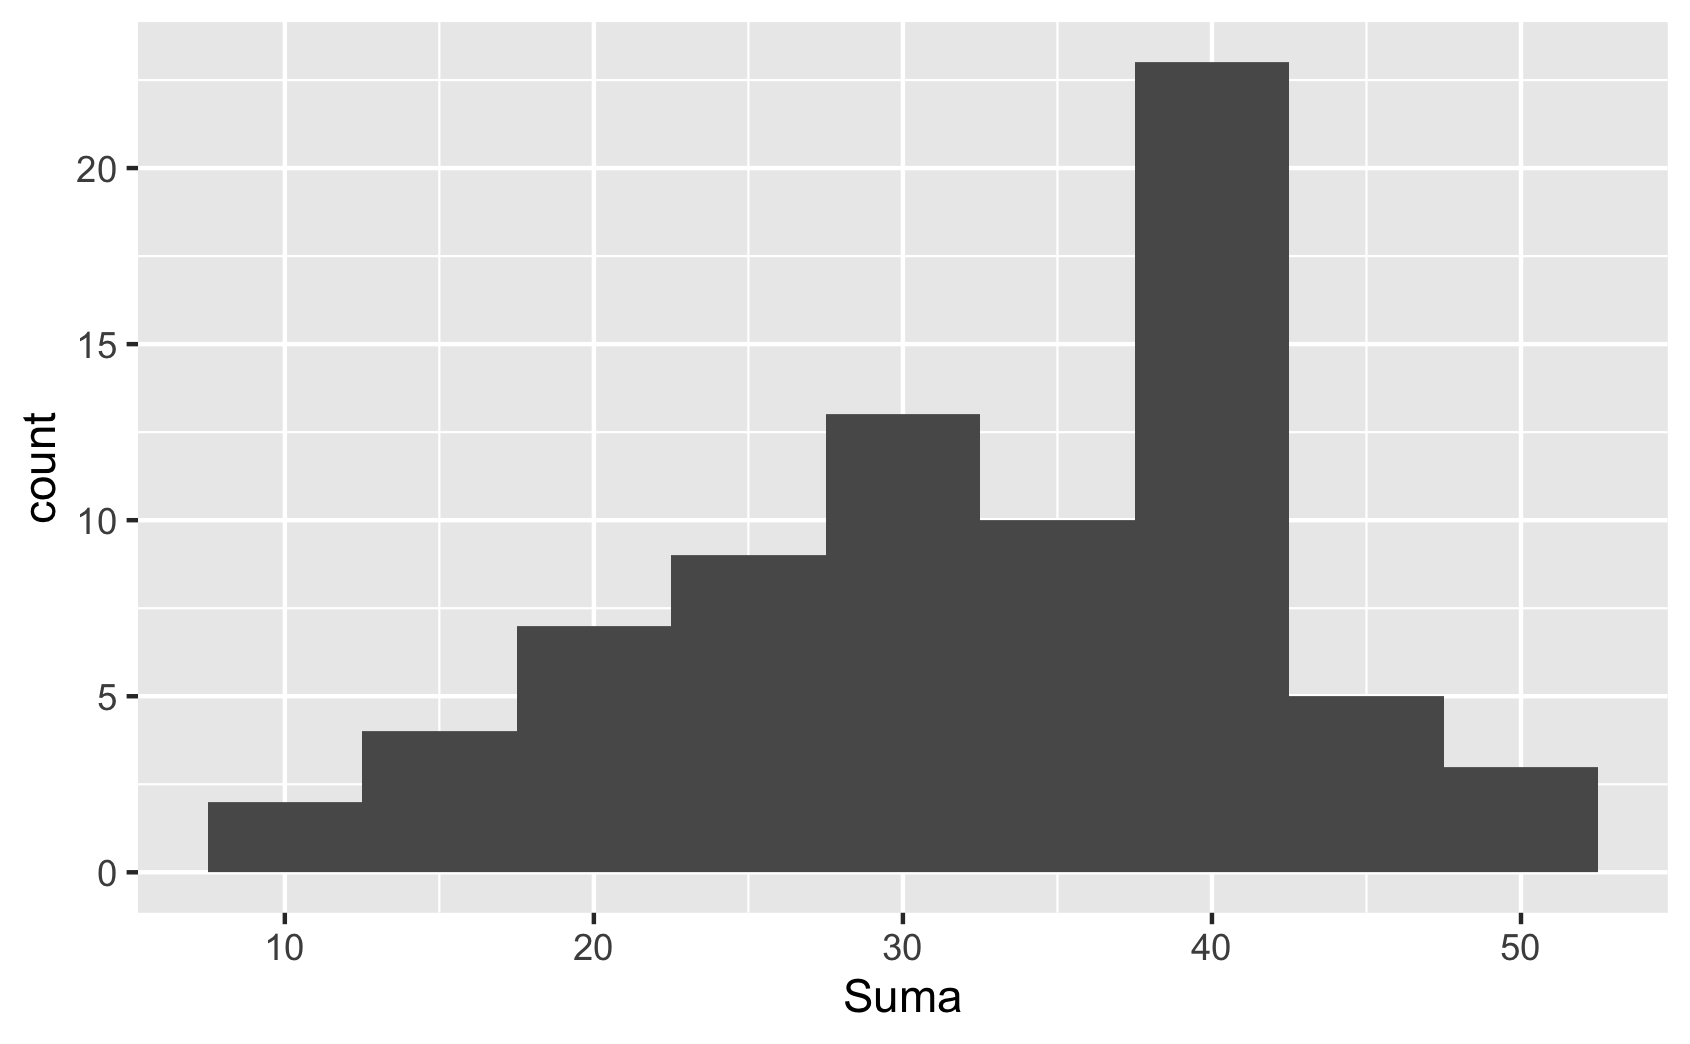
\includegraphics[scale=0.2]{histogram_all}
\end{figure}
\section*{\large{\textbf{\textsc{Wyniki}}}}
\paragraph{}
Po sprawdzeniu normalności rozkładu i na tej podstawie wyboru testu statystycznego obliczone zostały podstawowe statystyki opisowe dla obu grup. Były to miary tendencji centralnej - średnia oraz mediana, jak również miary zróżnicowania - odchylenie standardowe oraz rozstęp. Wyniki podstawowych działań statystycznych zostały przedstawione w \textit{tabeli 1}. \\
\begin{table}[h!]
\caption{\textit{Wyniki podstawowych parametrów statystyki opisowej}}
\begin{tabular}{lccccccc}
\textbf{Modyfikacja} & \textbf{N}                                        & \textbf{Średnia}                                    & \textbf{Mediana}                                    & \textbf{\begin{tabular}[c]{@{}c@{}}Odchylenie\\ Standardowe\end{tabular}} & \textbf{Max}                                      & \textbf{Min}                                      & \textbf{Rozstęp}                                  \\
Tak                  & {\color[HTML]{333333} 25}                         & {\color[HTML]{333333} 32.7}                         & {\color[HTML]{333333} 32}                          & {\color[HTML]{333333} 9.6}                                                 & {\color[HTML]{333333} 49}                         & {\color[HTML]{333333} 11}                         & {\color[HTML]{333333} 38}                         \\
Nie                  & \cellcolor[HTML]{F2F2F2}{\color[HTML]{333333} 51} & \cellcolor[HTML]{F2F2F2}{\color[HTML]{333333} 32.7} & \cellcolor[HTML]{F2F2F2}{\color[HTML]{333333} 34} & \cellcolor[HTML]{F2F2F2}{\color[HTML]{333333} 9.59}                         & \cellcolor[HTML]{F2F2F2}{\color[HTML]{333333} 50} & \cellcolor[HTML]{F2F2F2}{\color[HTML]{333333} 11} & \cellcolor[HTML]{F2F2F2}{\color[HTML]{333333} 39}
\end{tabular}
\end{table}
\paragraph{}
Poza podstawowymi miarami rozkładu wyników, policzone zostały testy statystyczne wskazujące na ewentualne zależności pomiędzy porównanymi grupami. Wartość \textit {p} testu t studenta z poprawką Welcha wyniosła \textit{p = 0.9912}. Następnie sprawdzony został ,,stopień do jakiego badane zjawisko istnieje’’ \citep[s. 5]{cohen_statistical_1977} za pomocą współczynnika d Cohena, którego wartość wyniosła 0.002698416. Aby wizualnie przedstawić porównanie badanych grup, na podstawie obliczonych parametrów został stworzony wykres pudełkowy, który przedstawiony jest na \textit{Rysunku 2}.
\begin{figure}[h!]
\caption{\textit{Wykres pudełkowy porównujący badane grupy}}
\centering
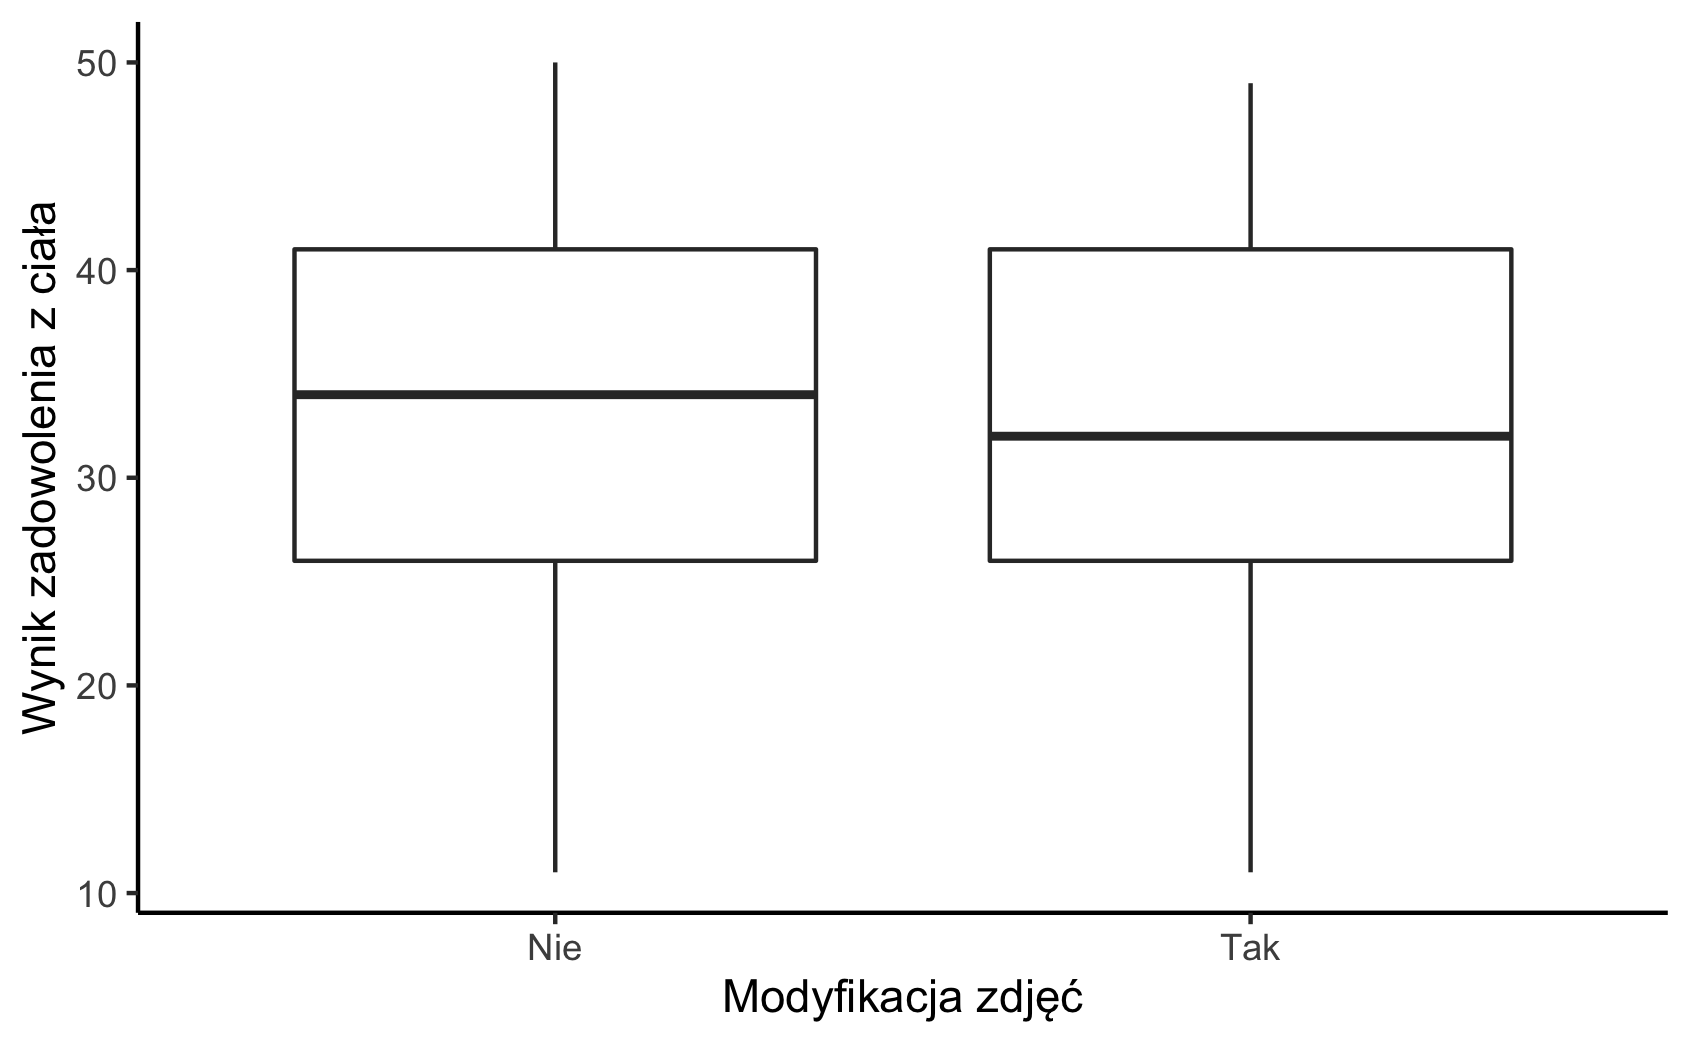
\includegraphics[scale=0.19]{boxwhisk}
\end{figure}
\paragraph{}
Hipoteza postawiona w całym badaniu została przyjęta jako \textit{Hipoteza zerowa (H$_0$)} w analizie statystycznej testującej hipotezy, zaś \textit{Hipoteza alternatywna (H$_1$)} jest zaprzeczeniem \textit{H$_0$}. Z tego względu wynik testu t studenta został porównany z przyjętym poziomem istotności. Po porównaniu wartości \textit{p} można pokazać, że \textit{H$_0$} musi zostać odrzucona, zaś \textit{Hipoteza alternatywna} została przyjęta. Siła zaobserwowanego efektu d Cohena jest mniejsza od 0.2 i jest bliska zera co wskazuje na brak występowania efektu pomiędzy grupami.
\section*{\large{\textbf{\textsc{Dyskusja}}}}
\newpage
\bibliography{BB}
\end{document}